\chapter{Several variable differential calculus}
\section{Linear transformation}
\paragraph{Excercise 6.1.43.}
\begin{proof}
\[(L_{AB}x)\trans=ABx\trans=A(L_{B}x)\trans=(L_{A}(L_{B}x))\trans
\]
Hence, $L_{A}L_{B}=L_{AB}$
\end{proof}
\section{Derivatives in several variable caculus}
\paragraph{Excercise 6.2.1.}
\begin{proof}With a little bit arrangement, the following inequality can be got.
\[\|\frac{f(x_{0}+tv)-f(x_{0})}{t}-L_{1}(v)\|<\varepsilon\]
\[\|\frac{f(x_{0}+tv)-f(x_{0})}{t}-L_{2}(v)\|<\varepsilon\]
\begin{figure}[H]
\centering
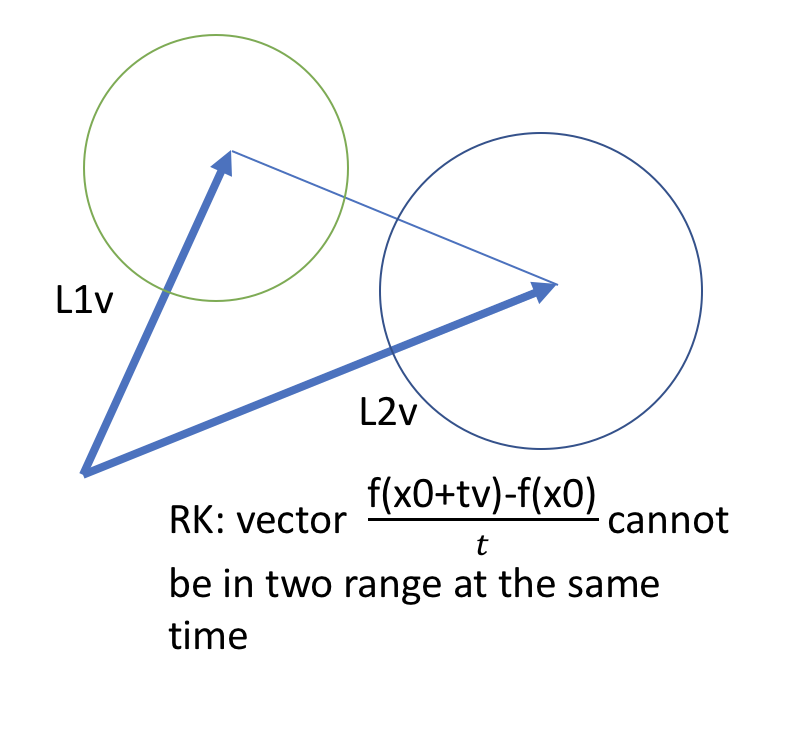
\includegraphics[width=8cm]{Uniqueness_Of_Derivatives}
\caption{Range of vector $\frac{f(x_{0}+tv)-f(x_{0})}{t}$}
\end{figure}
Pick $\varepsilon$ careful enough($<\|\frac{L_{1}(v)-L_{2}(v)}{2}\|$), we can make the contradiction.
\end{proof}
\section{Partial and directional derivatives}
\paragraph{6.3.3.}The big idea is that the partial derivatives all exists at (0,0) but it isn't continuous at (0,0). Also, it is not differentiable at(0,0).
Take partial derivative of second variable as an example. It is easy to check that $\frac{\partial f}{\partial y}(0,0)=0$
\begin{align}
\frac{\partial f}{\partial y}(t_{1},t_{2})&=\lim_{t\rightarrow 0}\frac{f(t_{1},t_{2}+t)-f(t_{1},t_{2})}{t}
\\&=\lim_{t\rightarrow 0}\frac{t_{1}^3}{(t_{1}^2+t_{2}^2)}\frac{(-2t-2t_{2})}{(t_{1}+t_{2}^2+4tt_{2}+3t^2)}\\
&=\frac{-2t_{1}^3t_{2}}{(t_{1}^2+t_{2}^2)^2}
\end{align}
When $t_{1}=t_{2}$ and they both go to zero,
\[\lim_{(t_{1},t_{2})\rightarrow (0,0)}\frac{\partial f}{\partial y}(t_{1},t_{2})=-\frac{1}{2}\neq0\]
From above, it is clear that the partial derivative exists but not continuous. Therefore, it doesn't contradict Theorem 6.3.8. I think $\frac{\partial f}{\partial x}$ is something similiar which is left to readers. (While, I haven't done it.)\\Now let's prove why it is not differentiable.
\begin{proof}
We want to show for any Linear transformation $L$. There exists a $\varepsilon$ s.t. for any $\delta$ there exists a point near (0,0) within $\delta$ (which is to say $\sqrt{x^2+y^2}\leq\delta$) satisfies:
\[\frac{\|f(x,y)-f(0,0)-L(x,y)\|}{\|(x,y)\|}>\varepsilon
\]
which is same as to prove there always exists (x,y) s.t.
\[|\frac{x^3}{x^2+y^2}\frac{1}{\sqrt{x^2+y^2}}-\frac{A(x,y)\trans}{\sqrt{x^2+y^2}}|>\varepsilon
\]
(Linear transformation $L$ is equivalent to matrix $A=(a,b)$)
\[|(\frac{x}{\sqrt{x^2+y^2}})^3-\frac{(a,b)(x,y)\trans}{\sqrt{x^2+y^2}}|>\varepsilon
\]
\[|cos(\alpha)^3-acos(\alpha)-bsin(\alpha)|>\varepsilon
\]
With the change of variable, it is more clear that for any given $a, b$ there exist a $cos(\alpha)$ to hold the inequality ( with $\|(x,y)\|<\delta$). Although the proof is not that rigorous for we didn't find the $\varepsilon$, this is more intuitively than before.
\end{proof}
\paragraph{\textcolor{red}{Excercise 6.3.4.}} Maybe we should treat component of function $f$ seperately. After constructing a function $\phi_{1}(t): \mathbb{R}\rightarrow\mathbb{R} := f_{1}(x+t(x^\prime-x))$, we can use MVT. To show that $f_{1}(x)=f_{1}(x^\prime)$. When the domain $\mathbb{R}^n$ is replaced by an open connected subset $\Omega$ of $\mathbb{R}^n$, I didn't see any differences.

\section{The several variable calculus chain rule}
\paragraph{Excercise 6.4.1} Let $A$ be the matrix representation of linear transformation $T$. $T^\prime=A$
The reason is:
\[\|Ax-A_{x_{0}}-A(x-x_{0})\|=0<\varepsilon
\]
Also $DT=A$
\paragraph{Excercise 6.4.2} A function $f$ is differentiable at $x_{0}$, then there exist a \emph{linear transformation} $f^\prime(x_{0})$ satisfies the following:
\[\|f(x)-f(x_{0})\|\leq\|f(x)-f(x_{0})-f^\prime(x_{0})(x-x_{0})\|+\|f^\prime(x_{0})(x-x_{0})\|\leq\varepsilon\|x-x_{0}\|+M\|x-x_{0}\|
\]
The inequality of right hand side is because of excercise6.1.4.
Because of the inequality, indeed, it is continuous.
\paragraph{Excercise 6.4.3}\begin{proof}Clarification:\\
The goal is to show that every sequence which converges to $x_{0}$ has the property that:
\[\lim_{x\rightarrow x_{0}}\frac{\|(g\circ f)(x)-(g\circ f)(x_{0})-g^\prime(f(x_{0}))f^\prime(x_{0})(x-x_{0})\|}{\|x-x_{0}\|}=0
\]
What we have is function $g$ is differentiable at $f(x_{0})$ which means:
\begin{equation}\label{a}
\lim_{y\rightarrow f(x_{0})}\frac{\|g(y)-g(f(x_{0}))-g^\prime(f(x_{0}))(y-f(x_{0}))\|}{\|y-f(x_{0})\|}
\end{equation}
Also, fucntion $f$ is differentiable at $x_{0}$:
\begin{equation}\label{b}
\lim_{x\rightarrow x_{0}}\frac{\|f(x)-f(x_{0})-f^\prime(x_{0})(x-x_{0})\|}{\|x-x_{0}\|}
\end{equation}
When $x\rightarrow x_{0}; f(x)\rightarrow f(x_{0})$, by excercise 6.4.2. Therefore, \ref{b} can be expressed as:
\[\lim_{x\rightarrow x_{0}}\frac{\|g(f(x))-g(f(x_{0}))-g^\prime(f(x_{0}))(f(x)-f(x_{0}))\|}{\|f(x)-f(x_{0})\|}=0
\]
%Let's say it is $a_{1}=\lim_{x\rightarrow x_{0}}\frac{\|g(f(x))-g(f(x_{0}))-g^\prime(f(x_{0}))(f(x)-f(x_{0}))\|}{\|f(x)-f(x_{0})\|}=0$ for short.\\
From excercise 6.4.2. we know that $\exists$ constant $M$ s.t. $\|f(x)-f(x_{0})\|<M\|x-x_{0}\|$\\
Therefore,
\begin{equation}\label{d}\lim_{x\rightarrow x_{0}}\frac{\|g(f(x))-g(f(x_{0}))-g^\prime(f(x_{0}))(f(x)-f(x_{0}))\|}{\|x-x_{0}\|}=0
\end{equation}
With \ref{a}, we can get
\begin{align}
0\leq&\label{c}\lim_{x\rightarrow x_{0}}\frac{\|-g^\prime(f(x_{0}))f^\prime(x_{0})(x-x_{0})+g^\prime(f(x_{0}))(f(x)-f(x_{0}))\|}{\|x-x_{0}\|}\\\\
\leq&\lim_{x\rightarrow x_{0}}\frac{\|g^\prime((f(x_{0}))(f(x)-f(x_{0})-f^\prime(x_{0})(x-x_{0}))\|}{\|x-x_{0}\|}\\\\
\leq&\lim_{x\rightarrow x_{0}}\frac{\|g^\prime((f(x_{0}))\|\|f(x)-f(x_{0})-f^\prime(x_{0})(x-x_{0})\|}{\|x-x_{0}\|}=0
\end{align}
Add \ref{c} to \ref{d}, we get the target.
\end{proof}






